\chapter{Град Киев близ Юрковицы}

Сейчас мне важно важно ввести предположение,  
 что первоначальный град Киев был в другом месте, нежели считают ученые. А именно – в окрестностях кирпичного завода у перекрестка улиц Кирилловской и Нижнеюрковской. Обоснования я дам развернуто в отдельной части книги, про Кирилловские высоты.

Давайте разберем хрестоматийные слова Нестора в «Повести временных лет» (Ипатьевский список):

\begin{quotation}  
Поляном же живущиим о собе и владеющим роды своими, яже и до сея братья бяху поляне, и живяху кождо с родом своим на своих местех, володеюще кождо родом своим. 

И быша 3 брата: а единому имя Кий, а другому Щек, а третьему Хорив, и сестра их Лыбедь. И седяше Кий на горе, кде ныне увоз Боричев, а Щек седяше на горе, кде ныне зовется Щековица, а Хорив на третьей горе, отнюду же прозвася Хоривица. Створиша городок во имя брата их старейшаго и нарекоша и Киев. 

И бяше около города лес и бор велик, и бяху ловяще зверь, бяхуть бо мудре и смыслени, и нарицахуся поляне, от них же суть поляне – кияне и до сего дни.

Инии же, не ведуще, ркоша, яко Кий есть перевозник бысть, у Киева бо перевоз бяше тогда с оноя страны Днепра, темь глаголаху: «На перевоз на Киев». Аще бо был перевозник Кый, то не бы ходил к Цесарюграду. 

Но сий Кий княжаше в роду своем, и приходившю ему к цесарю – не свемы, но токмо о сем вемы, якоже сказають: яко велику честь приял есть от цесаря, которого не вем и при котором приходи цесари. 

Идущю же ему опять, приде к Дунаеви, и возлюби место, и сруби городок мал, и хотяше сести с родом своим, и не даша ему близ живущии; еже и доныне наречють дунайци городище Киевець. 

Киеви же пришедшю в свой город Киев, ту и сконча живот свой, и брата его – Щек и Хорив, и сестра их Лыбедь ту скончашася.
\end{quotation}  

Прежде чем обсуждать замечу, что во времена Нестора (11-12 столетия) «градом», «городком» именовали огороженное селение того или иного размера, иначе говоря – крепость. Само по себе слово говорящее – град, город – городить. Посему, когда пишется, что кто-то сотворил или срубил град либо городок, это не значит, что раньше в том месте никто не жил и на пустоши вдруг основали селение. Нет, там просто возвели деревянную крепость. Глагол «срубили» на это еще яснее указывает, если только мы верно трактуем это слово.

«Срубили», конечно, легко и просто толковать как сооружение деревянных построек. Известно производное слово – «сруб», а «рубить» обычно применяется к дереву. Но что, если «срубили» сходно с украинским «зробили», то есть просто «сделали»? Ведь «робить» – работать. Срубили могло означать и «сработали». Слова со временем меняют значение. Например, когда в летописи говорится о каменной церкви, это значит, что она сделана из кирпича, а не составлена из каких-то вытесанных валунов. Вплоть до 19, начало 20 века под каменными домами подразумевались кирпичные.

Еще о срубе и хате. Так вышло, что хата представляется нам не иначе как «мазанкой». Но в основании ее, как у избы, лежат бревна, да и частью мазанки иногда был обычный бревенчатый сруб.

Слово «хата» в значении «дом» у ирландцев звучит похоже – «котта», близко к этому английское «cottage» и «hut» (домик, избушка). Но что означает оно? Каков смысл? Ключик находим в языках славянских.

Прямой перевод слова «рубить» на английский – «cut» («кат»). Кстати палач – «кат» – потому, что тоже рубит. Итак, «hut» или «cotta» – тот же «сруб», только наш сруб от «рубить», а их «hut» и «cotta[ge]» от того же «рубить», но в виде английского «cut».

Однако выйдем из области языковедения.

Итак, Нестор обосновывал в летописи такой вариант основания Киева – были некие Поляне, братья Кий, Хорив и Щек, да сестра их Лыбедь, обосновавшиеся тут, каждый со своим родом, на своем холме. Кий «сидел» – жил то бишь, на горе, где во время составления Нестором летописи был увоз Боричев.

Про связь «увоза» с предположением, что Кий был перевозчиком на речной переправе, мы подробно поговорим в главах об увозе Боричевом. Пока скажу, что Кий поселился на холме, известном ныне как Старокиевский. Насколько землями Кия считались примыкающие горбы да отроги – горы Андреевская, Уздыхальница, Клинец и Замковая (Киселёвка, Флоровская) – сказать точно затрудняюсь. 

В цитате, летописец никак не называет гору жительства Кия. Ни Киевица, ни конечно же Старокиевская, но просто обозначает – где ныне Увоз Боричев. Впрочем, Киевица есть в списках: «И вселися Кий на горе, яже нарицается Киевица». Делаем вывод, что гора с Увозом Боричевым и есть Киевица.

На одной из соседних гор – Щекавице – зажил Щек, а вот Хоривица (в некоторых списках Хор\textbf{е}вица) брата Хорива в летописях отражена, но не указано ея расположение, поэтому Хоривицей могли называть как соседние горы вроде Киселёвки, так и отдаленные, что поныне служит предметом споров. Если именование Щекавицы сохранилось, то Хоривица стёрлась в памяти людской, хотя есть соображения на этот счет – что не совсем стёрлась, а преобразилась в Юрковицу, ибо Хорив, мол, это Оурив, он же Юрий. Но про это позже.

Три брата «сотворили» городок и назвали его в честь старшего – Киев. Чей городок? А Киев! Кстати, в годы те стародавние, местные жители вероятно произносили не Киев, но Кыев. И Кый вместо Кий. Говорили не «хан», но «кан» (например, Тугоркан – это хан Тугор), отсюда название города Канев. То есть, чей? А канев, «ханов».

Теперь пойдет ересь.

А где братья сотворили городок в честь Кия? Несколько веков бытует ответ – где сидел Кий, там и сотворили. Вот же, рядом потом вроде и терем княгини Ольги был, и археологи раскопали остатки княжеского дворца, ну и оттуда разрастался град Киев... Всем известно...

Но задам другой вопрос – а разве в летописи сказано, где именно братья сотворили городок? Быть может, в седую старину была иная трактовка летописи? Оказывается да.

Я покажу вам интересную картинку из Радзивилловской летописи. Вот как иллюстрирует художник поселение братьев на горах:

\begin{center}
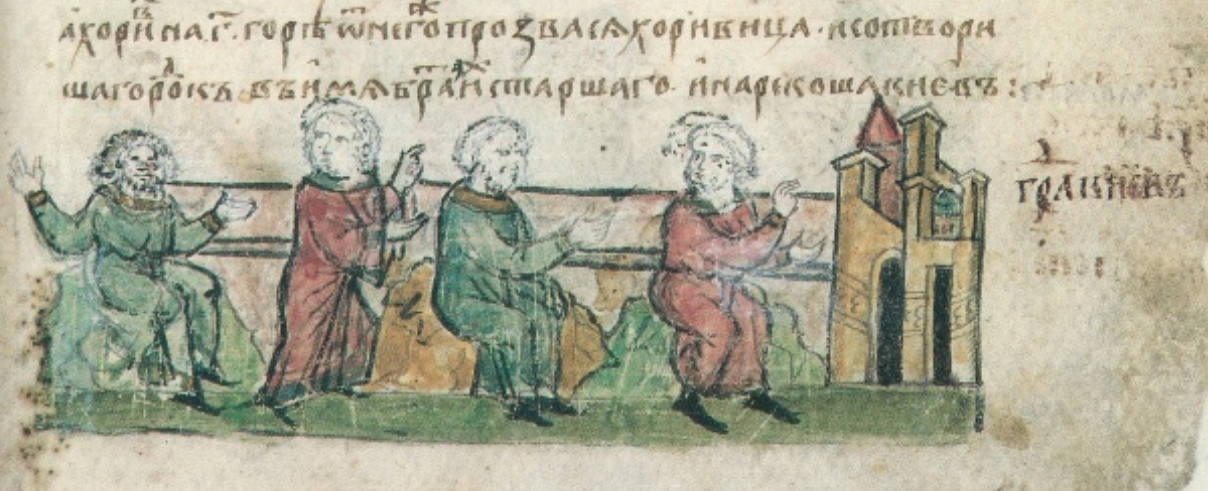
\includegraphics[width=\linewidth]{chast-colebanie-osnov/grad-kiev-urk/radz-tri-brata.jpg}
\end{center} 

Художник буквально усадил братьев на холмы. Самый бородатый да патлатый, старший – слева, на зеленой горе – Кий. Правее от него, круглолицая и безбородая стоит, наверное, Лыбедь. Затем, справа от нее, на желтой горе сидит второй брат. И на следующей зеленой – третий. И за ними еще правее нарисован условно град, после чего еще написано для ясности: «ГРАКИЕВЪ» («д» приписана сверху над «р»).

Ой-ёй-ёй! Может быть художник просто всё с кондачка нарисовал! Град Киев надо было с другой стороны, возле Кия!

А теперь давайте серьезно. Видите эту широкую линию, которая идет за братьями? Это река Лыбедь. Видите холм с крутым склоном, на коем восседает Кий? Это край Замковой горы. Видите желтую гору? Это Щекавица. Правее зеленая гора – Хоривица, которая, как обосную в этой книге позже, ныне считается отрогом Щекавицы со Старообрядческим кладбищем.

Рисунок из Радзивилловской летописи расположением холмов точно соответствует действительному, как это выглядит с левого берега Днепра.

Художник Абрахам ван Вестерфельд в 1651 году запечатлел известную панораму правого берега Киева. Вот она на копии рисунка – правда, крайняя справа гора не поместилась, видна лишь часть склона. Тот же рельеф, последовательно, слева направо: Замковая – удолье – Щекавица – овраг.
 
\begin{center}
\includegraphics[width=\linewidth]{chast-colebanie-osnov/grad-kiev-urk/\myimgprefix vester-02.jpg}
\end{center} 

А вот о Хоривице разговор особый. Да, еще - почему я пишу Хоривица, а не Хоревица? Потому что одного из братьев звали Хорив. В некоторых списках гора Хоревица, в иных Хоривица. Я выбираю последнее.

Далее, в части про Кирилловские высоты, я подробно опишу модель развития именований на местности, из которой следует, что современная гора Юрковица на картах носит это название ошибочно. Прежде эта гора, когда была менее съедена кирпичными заводами, называлась Лысой. В Киеве вообще много Лысых гор, но эта возникает в земельных документах первой.

А Юрковица - покамест голосовно сопоставлю ее с Хоривицей, то есть с отрогом Щекавицы за старообрядческим кладбищем. 

На остатках же той Лысой горы на Кирилловских высотах, сохранились древние валы укреплений, следы старинных земляных работ по фортификации, да и остатки строений «великокняжеского» времени. Профессор Антонович нашел на склоне её останки 4000 тысяч людей, что возможно свидетельствует о большом поселении и большой гибели.

Существует большая вероятно, что первоначальный «град Киев» (не место, где жил Кий, а общая для братьев крепость) располагался на Кирилловских высотах, а не, как считают, на Старокиевской горе. Кий мог даже не переселяться в «град» и жить по прежнему адресу.

У подножия юго-западного склона Замковой, в урочище Кожемяки, протекала река Киянка, ныне взятая в коллектор – вот еще одна память о близости к обитанию Кия.

Но вернемся к летописи. Далее по Нестору, около города были дремучий лес и бор со зверями, а Поляне стали именоваться Киянами. Чьи вы люди, какого роду? А Кия! Кияне. «И бяше около города лес и бор велик, и бяху ловяще зверь».

Обычно думают, что Нестор говорил об урочище «перевесище» (место охоты перевесом – сетью), упомянутом в летописи позже, в разделе о княгине Ольге. Где было перевесище? Одни считают, что это участок между нынешними Европейской и Независимости площадями. Иные – что находилось где Владимирская горка и почти весь Крещатик. Проще предполагать, чем признаться в неведении. А на плане Киева 1860 года Перевесище обозначено на отрезке от низа Шелковичной до начала Жандарской (Саксаганского), то есть удолье с Дворцом спорта.

%А «перевесище», бают ученые, от слова «перевес» – сеть на мелкого зверя. 


%Но перевесище это еще и пропускной пункт со шлагбаумом.

Но ежели мы примем ересь о Киеве и будем рассуждать не о перевесище, но лишь о том, что говорит летописец – о каком-то лесе и боре великом около града – то этот лес может оказаться совсем в другой стороне.

Бор это хвойный, корабельный лес. Лесом же называли лиственные леса. Где какие леса и боры были в те времена, может и показали бы некие раскопки. 

Например, возле нынешней Лавры, по словам Нестора, «бе бо лес ту велик». Закревский во втором томе «Описания Киева»\cite{zakr01}, рассказывая про окрестности урочища Юрковицы, о склонах, вскользь упоминает: «но по местам видны и одиноко растущие высокие сосны». На дореволюционных снимках можно видеть сосны и около Заведения искусственных минеральных вод под Владимирским спуском, и за Михайловским собором, в сторону Владимирской горки.

Нестор приводит также другой вариант основания Киева – мол, был такой перевозчик через Днепр – Кий, и люди говорили  «на перевоз на Киев». Нестор рассуждает, основываясь на каких-то своих источниках, что Кий являлся князем, главным среди братьев, и ходил к цесарю в Царьград – и вряд ли такое затеял бы простой перевозчик. 

Нестор, размышляя вслух, держит в уме источник, не вошедший в «Повесть временных лет». Кроме того, Нестор не пишет, к какому именно цесарю ходил Кий. Эта неопределенность развязывает руки воображению. Цесарей было много, жили в разное время.

Археолог и историк, академик Борис Рыбаков, долгие годы задававший тон советской истории да археологии, вытянул из забвения имя византийского военного деятеля Хильбудия, найдя в его судьбе сходство с Кием, что позволило отодвинуть предание о последнем ко времени императора Юстиниана (527-565) – либо, по другим работам ученого – к императору Анастасию (491-518 годы)\footnote{А в 1918 году на улице Ивановской, ныне Тургеневской, нашли серебряную монету Александра Македонского.}. Мол, тогда византийцы нанимали славянские дружины и селили их по Дунаю, чтобы те в случае чего пособили Царьграду против Гуннов.

Менялись слова Рыбакова, ходил вокруг да около, но прямо Кия с Хильбудием не отождествлял. Когда два слова трутся друг о друга, всё время рядом, кто-то возьмет да сопоставит.
